%%%  Ukázkový text a dokumentace stylu pro text závěrečné (bakalářské a
%%%  diplomové) práce na KI PřF UP v Olomouci
%%%  Copyright (C) 2012 Martin Rotter, <rotter.martinos@gmail.com>
%%%  Copyright (C) 2014 Jan Outrata, <jan.outrata@upol.cz>


%%  Pro získání PDF souboru dokumentu je třeba tento zdrojový text v
%%  LaTeXu přeložit (dvakrát) programem pdfLaTeX.

%%  V případě použití programu BibLaTeX pro tvorbu seznamu literatury
%%  je poté ještě třeba spustit program Biber s parametrem jméno
%%  souboru zdrojového textu bez přípony a následně opět (dvakrát)
%%  přeložit zdrojový text programem pdfLaTeX.

%%  Postup získání Postscriptového souboru je popsán v dokumentaci.


%%  Třída dokumentu implementující styl pro závěrečnou práci. Vybrané
%%  nepovinné parametry (ostatní v dokumentaci):

%%  'master' pro sazbu diplomové práce, jinak se sází bakalářská práce

%%  'program=kód' pro Váš studijní program/obor (specializaci), kódy
%%  pro diplomovou práci 'infoi' pro Informatiku (Obecná informatika),
%%  'infui' pro Informatiku (Umělá inteligence), 'ainfpst' pro
%%  Aplikovanou informatiku (Počítačové systémy a technologie), 'uinf'
%%  pro Učitelství informatiky pro střední školy, 'binf' pro
%%  Bioinformatiku, 'inf' pro Informatiku (bez specializací) a 'ainf'
%%  pro Aplikovanou informatiku (bez specializací), jinak je výchozí
%%  ainfvs pro Aplikovanou informatiku (Vývoj software), a pro
%%  bakalářskou práci 'infoi' pro Informatiku (Obecná informatika),
%%  'itp' pro Informační technologie v prezenční formě, 'itk' pro
%%  Informační technologie v kombinované formě, 'infv' pro Informatiku
%%  pro vzdělávání, 'binf' pro Bioinfomatiku, 'inf' pro Informatiku
%%  (bez specializací), 'ainfp' pro Aplikovanou informatiku (bez
%%  specializací) v prezenční formě, 'ainfk' pro Aplikovanou
%%  informatiku (bez specializací) v kombinované formě, jinak je
%%  výchozí infpvs pro Informatiku (Programování a vývoj software)

%%  'printversion' pro sazbu verze pro tisk (nebarevné logo a odkazy,
%%  odkazy s uvedením adresy za odkazem, ne odkazy do rejstříku),
%%  jinak verze pro prohlížeč

%%  'biblatex' pro zapnutí podpory pro sazbu bibliografie pomocí
%%  BibLaTeXu, jinak je výchozí sazba v prostředí thebibliography

%%  'language=jazyk' pro jazyk práce, jazyky english pro anglický,
%%  slovak pro slovenský, jinak je výchozí czech pro český

%%  'font=sans' pro bezpatkový font (Iwona Light), jinak je výchozí
%%  serif pro patkový (Latin Modern)

%%  'figures, tables, theorems a sourcecodes' pro sazbu seznamu
%%  obrázků, tabulek, vět a zdrojových kódů, jinak při =false se
%%  nesází (u theorems a sourcecodes výchozí)

\documentclass[
%  master,
%  program=ainfvs,
%  printversion,
  biblatex,
%  language=english,
%  font=sans,
  figures,
  tables,
%  theorems,
%  sourcecodes,
  glossaries,
  index
]{kidiplom}

\addbibresource{bibliografie.bib}

%% Informace pro úvodní strany. V jazyku práce (pokud není v komentáři
%% uvedeno česky) a anglicky. Uveďte všechny, u kterých není v
%% komentáři uvedeno, že jsou volitelné. Při neuvedení se použijí
%% výchozí texty. Text pro jiný než nastavený jazyk práce (nepovinným
%% parametrem language makra \documentclass, výchozí český) se zadává
%% použitím makra s uvedením jazyka jako nepovinného parametru.

%% Název práce, česky a anglicky. Měl by se vysázet na jeden řádek.
\title{Nástroj pro automatickou kontrolu programátorských úkolů}
\title[english]{Automated checker for programming assignments}

%% Jméno autora práce. Makro nemá nepovinný parametr pro uvedení
%% jazyka.
\author{My Linh Duongová}

%% Jméno vedoucího práce (včetně titulů). Makro nemá nepovinný
%% parametr pro uvedení jazyka.
\supervisor{Mgr. Petr Osička, Ph.D.}

%% Volitelný rok odevzdání práce. Výchozí je aktuální (kalendářní)
%% rok. Makro nemá nepovinný parametr pro uvedení jazyka.
%\yearofsubmit{\the\year}

%% Anotace práce, včetně anglické (obvykle překlad z jazyka
%% práce). Jeden odstavec!
\annotation{Automatizované vyhodnocování programátorských úloh představuje způsob, jak zefektivnit proces hodnocení zdrojových kódů a omezit potřebu manuální kontroly v~náborových procesech vývojářů. Tato bakalářská práce se zabývá návrhem a implementací modulárního systému pro automatické zpracování GitHub repozitářů, spuštění nedůvěryhodného zdrojového kódu v~izolovaném kontejnerovém prostředí a sběr výsledků vyhodnocení. Výstupem práce je funkční prototyp systému pro automatizované vyhodnocování úkolů s~důrazem na bezpečnost, modularitu a snadnou rozšiřitelnost o~další programovací jazyky.}


\annotation[english]{Automated evaluation of programming assignments represents a way to streamline the source code evaluation process and reduce the need for manual review in developer recruitment processes. This bachelor’s thesis deals with the design and implementation of a modular system for automatic processing of GitHub repositories, execution of untrusted source code in an isolated container environment and collection of evaluation results. The output of this thesis is a functional prototype of a system for automated assignment evaluation, with an emphasis on security, modularity and easy extensibility to support additional programming languages.}


%% Klíčová slova práce, včetně anglických. Oddělená (obvykle) středníkem.
\keywords{automatizované testování, Podman, kontejnerizace, GitHub~API, RabbitMQ}
\keywords[english]{automated testing, Podman, containerization, GitHub~API, RabbitMQ}

%% Volitelná specifikace příloh textu práce, i anglicky. Výchozí je
%% 'elektronická data v systému katedry informatiky / electronic data
%% in system of department of computer science'.
%\supplements{nejlepší software všech dob}
%\supplements[english]{the best software of all times}

%% Volitelné poděkování. Stručné! Výchozí je prázdné. Makro nemá
%% nepovinný parametr pro uvedení jazyka.
\thanks{TODO: Děkuji, děkuji, děkuji.}

%% Cesta k souboru s bibliografií pro její sazbu pomocí BibLaTeXu
%% (zvolenou nepovinným parametrem biblatex makra
%% \documentclass). Použijte pouze při této sazbě, ne při (výchozí)
%% sazbě v prostředí thebibliography.
\bibliography{bibliografie.bib}

%% Další dodatečné styly (balíky) potřebné pro sazbu vlastního textu
%% práce.
\usepackage{lipsum}
\usepackage{longtable}
\usepackage{float}

\begin{document}
%% Sazba úvodních stran -- titulní, s bibliografickými údaji, s
%% anotací a klíčovými slovy, s poděkováním a prohlášením, s obsahem a
%% se seznamy obrázků, tabulek, vět a zdrojových kódů (pokud jejich
%% sazba není vypnutá).
\maketitle

%% Vlastní text závěrečné práce. Pro povinné závěry, před přílohami,
%% použijte prostředí kiconclusions. Povinná je i příloha s obsahem
%% elektronických dat.

%% -------------------------------------------------------------------

\newcommand{\BibLaTeX}{\textsc{Bib}\LaTeX}

% \noindent\textcolor{red}{\LARGE Upozornění: Následující text
%   dokumentace stylu, vyjma přílohy~\ref{sec:ObsahData}, je rozpracovaná
%   a (značně) neúplná verze!!!}

\section{Úvod}
Firma Edhouse~\cite{edhouse}, zabývající se vývojem softwaru a hardwaru, přijímá každým rokem nové stážisty. Součástí přijímacího řízení je praktické ověření znalostí, v~jehož rámci společnost poskytne zájemci zadání úkolu a ten následně vypracuje své řešení ve svém preferovaném programovacím jazyce.

S~rostoucím počtem uchazečů se ale tento proces setkal s~kapacitními omezeními. Odevzdaná řešení byla nejednotná. Lišila se adresářovou strukturou projektů anebo verzemi použitých jazyků. Vyhodnocování úkolů vyžadovalo manuální zásah mentorů, kteří museli zdrojové kódy ručně stahovat, nastavovat lokální prostředí, řešit závislosti a kód spouštět.

Vedle vysoké časové náročnosti, která prodlužovala délku náborového procesu a odváděla vývojáře od jejich primární práce, představovalo spouštění cizího a nedůvěryhodného kódu přímo na vývojářských prostředích bez dostatečné izolace rovněž bezpečnostní riziko pro interní infrastrukturu. Odlišnosti v~lokálním nastavení počítačů jednotlivých mentorů také mohly vést k~nekonzistentním výsledkům při kompilaci a spouštění řešení.

Hlavní motivací pro vznik platformy \textbf{InQuest} je proto ucelená automatizace prvotní fáze vyhodnocování úkolů. Systém standardizuje proces tím, že vyžaduje sjednocenou adresářovou strukturu odevzdávaných úkolů. Dále zajišťuje autonomní stažení kódu, jeho verifikaci a především izolované spuštění v~izolovaném kontejnerovém prostředí. Díky této automatizaci jsou mentoři odproštěni od repetitivních úkonů a mohou se soustředit na architekturu řešení, čistotu kódu a celkovou kvalitu návrhu.


\subsection{Analýza existujících řešení}
Automatizované vyhodnocování programátorských úloh představuje běžnou součást náborových procesů v~technologických společnostech i výuky na vysokých školách. V~současnosti existuje řada komerčních i open-source systémů, které umožňují automatické sestavení, spuštění a vyhodnocení zdrojových kódů. Tyto systémy se liší zejména mírou konfigurovatelnosti, podporovanými programovacími jazyky, způsobem izolace běhového prostředí a možnostmi integrace do dalších informačních systémů.

Cílem této kapitoly je představit existující platformy, zhodnotit jejich architekturu i omezení a identifikovat vlastnosti, které byly zohledněny při návrhu systému implementovaného v~této práci.


\subsubsection{HackerRank}
HackerRank je komerční platforma využívaná zejména při technických pohovorech, náborových akcích a online programátorských soutěžích. Uchazeč řeší zadané úlohy přímo ve webovém prostředí, přičemž systém automaticky provádí kompilaci, spuštění programu a vyhodnocení výsledků vůči připraveným testovacím sadám.~\cite{hackerrank}

Platforma podporuje desítky programovacích jazyků a nabízí pokročilé nástroje pro správu náborových procesů, tvorbu úloh i sledování výsledků kandidátů. Jedná se však o~uzavřené komerční řešení, které neumožňuje vlastní implementaci pokročilé validační logiky, přímé napojení na interní repozitáře firmy ani snadné rozšíření o~specifické požadavky organizace bez vysokých licenčních poplatků.


\subsubsection{CodeRunner}
CodeRunner je volně dostupné rozšíření pro výukový systém Moodle, které slouží k~automatickému hodnocení programátorských úloh. Vyhodnocení probíhá spuštěním řešení studenta v~izolovaném prostředí (sandboxu) a porovnáním výstupu s~očekávanými výsledky nebo pomocí vlastních unit testů.~\cite{coderunner}

Výhodou systému je jeho vysoká míra konfigurovatelnosti, otevřený zdrojový kód a široká podpora programovacích jazyků. Hlavní nevýhodou je však jeho úzká vazba na prostředí Moodle, což značně omezuje jeho využití v~podnikovém prostředí mimo oblast elektronického vzdělávání. Systém navíc primárně zpracovává jednotlivé kódové fragmenty, nikoli ucelené projekty se složitější adresářovou strukturou.


\subsubsection{Judge0}
Judge0 je open-source systém poskytující robustní REST~API pro kompilaci a spouštění zdrojových kódů v~izolovaných Docker kontejnerech. Podporuje velké množství programovacích jazyků a je častým stavebním kamenem pro vývoj vlastních online editorů či výukových platforem.~\cite{judge0}

Hlavní výhodou je otevřenost projektu, modulární architektura a jednoduché rozhraní. Na druhé straně systém nabízí pouze nízkoúrovňové spouštění jednotlivých skriptů. Neposkytuje nativní podporu pro stahování celých GitHub repozitářů, automatické určování použitého jazyka, kontrolu adresářové struktury projektu ani sestavení komplexnějších aplikací využívajících balíčkovací systémy (např. NuGet, npm nebo Maven).


\subsubsection{Shrnutí a porovnání analýzy}
Z~provedené rešerše vyplývá, že existující systémy poskytují kvalitní dílčí funkce, avšak jsou primárně navrženy buď pro akademické prostředí, nebo fungují jako uzavřené komerční platformy. Otevřená exekuční API (např. Judge0) sice nabízejí bezpečné spouštění izolovaného kódu, neřeší však ucelený proces automatického zpracování celých repozitářů odevzdaných uchazeči.

Klíčové vlastnosti a odlišnosti analyzovaných řešení jsou přehledně shrnuty v~tabulce~\ref{tab:srovnanisys}.

\begin{table}[H]
	\centering
	\small
	\begin{tabular}{|l|c|c|c|}
		\hline
		\textbf{Vlastnost / Systém} & \textbf{HackerRank} & \textbf{CodeRunner} & \textbf{Judge0} \\ \hline
		\textbf{Komerční řešení} & Ano & Ne & Ne  \\ \hline
		\textbf{Izolace} & Uzavřený Cloud & Sandbox & Docker kontejnery \\ \hline
		\textbf{Kontrola adresáře} & Ne & Ne & Ne \\ \hline
		\textbf{Vlastní zadání} & Omezená & Ano & Ano  \\ \hline
		\textbf{Podpora více jazyků} & Ano & Ano & Ano \\ \hline
	\end{tabular}
	\caption{Srovnání vlastností analyzovaných systémů}
	\label{tab:srovnanisys}
\end{table}

Jak ukazují data v~tabulce~\ref{tab:srovnanisys}, žádný ze stávajících systémů nenabízí automatizovanou kontrolu adresářové struktury odevzdaných projektů. Komerční nástroje neumožňují přímé napojení na interní vývojářské procesy a open-source alternativy se zaměřují pouze na spouštění jednotlivých skriptů či kódových fragmentů, nikoliv ucelených projektů s~vlastními závislostmi.


\subsection{Analýza problémů a požadavků}
Vyhodnocování úloh ve společnosti Edhouse probíhalo převážně ručně. Dalším problémem byl nejednotný způsob odevzdávání. Uchazeči zasílali svá řešení v~různých formátech a s~odlišnou strukturou projektu. Mentor musel odevzdané řešení stáhnout, připravit si odpovídající prostředí, projekt sestavit, spustit a následně zkontrolovat jeho výstup. Tento postup byl při větším počtu uchazečů časově náročný a zbytečně zatěžoval mentory. Bylo proto nutné stanovit jednotný způsob odevzdání, se kterým bude systém schopný dále pracovat bez ručních zásahů.

Požadavky na systém vycházely také z~průběhu náborového procesu. Komunikaci s~uchazeči zajišťuje především HR oddělení, proto musí být odeslání úlohy do systému co nejjednodušší. Uživatel by neměl potřebovat znalost vývojářských nástrojů ani provádět složitou konfiguraci. Základním vstupem má být pouze odkaz na odevzdaný repozitář.

Důležitou částí návrhu byla také bezpečnost. Odevzdané řešení obsahuje cizí zdrojový kód, který nelze považovat za důvěryhodný. Jeho spouštění přímo na pracovním počítači mentora by mohlo představovat riziko pro jeho stanici i interní síť. Z~tohoto důvodu bylo nutné zajistit oddělené prostředí pro spuštění jednotlivých úloh. Toto prostředí musí zároveň obsahovat nástroje potřebné pro konkrétní programovací jazyk a umožnit opakovatelné spuštění za stejných podmínek.

Systém musí být připraven také na budoucí rozšiřování. Podpora programovacích jazyků se může v~čase měnit, proto by přidání nového jazyka nemělo vyžadovat rozsáhlé změny v~ostatních částech aplikace. Tento požadavek ovlivnil především návrh architektury a způsob oddělení částí určených pro konkrétní programovací jazyky.

Z~provozního hlediska bylo požadováno, aby aplikace zvládala zpracovat více úloh současně. Vyhodnocování projektu může trvat delší dobu, a proto nesmí blokovat zpracování dalších požadavků ani nutit uživatele čekat na dokončení kontroly. Současně musí být zajištěno, že odevzdané úlohy a přístupové údaje k~repozitářům nebudou veřejně dostupné.

Z~uvedených problémů vyplynuly hlavní požadavky na nový systém: sjednocení způsobu odevzdávání, jednoduché použití, izolované spuštění cizího kódu, možnost paralelního zpracování a snadné rozšíření o~další programovací jazyky.


\subsection{Cíl práce}
Cílem bakalářské práce je navrhnout a implementovat systém InQuest pro automatizované vyhodnocování programátorských úloh. Systém má přijmout odkaz na odevzdaný GitHub repozitář, zjistit použitý programovací jazyk, spustit řešení v~izolovaném prostředí a uložit výsledek jeho vyhodnocení.

Navržené řešení má omezit množství ruční práce mentorů, sjednotit způsob odevzdávání úloh a umožnit zadání požadavku i pracovníkům HR oddělení bez nutnosti používat vývojářské nástroje. Zpracování úloh má probíhat asynchronně, aby delší sestavení nebo spuštění jednoho projektu neblokovalo ostatní požadavky.

Součástí práce je také návrh modulární architektury, která umožní přidávat podporu dalších programovacích jazyků bez výrazných zásahů do hlavní logiky aplikace. Výstupem práce je funkční prototyp systému ověřující navržený způsob zpracování programátorských úloh.

\newpage


\section{Použité technologie}
Při návrhu systému bylo nutné zvolit technologie, které umožní bezpečné spouštění cizího zdrojového kódu, asynchronní komunikaci mezi jednotlivými komponentami a snadné rozšiřování o~podporu dalších programovacích jazyků. Tato kapitola představuje použité technologie, důvody jejich výběru a jejich roli v~navrženém systému.


\subsection{\csharp{} | .NET}
Pro implementaci backendu byl vybrán jazyk \csharp{} na platformě .NET 8. Hlavními důvody byly podpora objektově orientovaného návrhu, silný typový systém, dostupnost nástrojů pro tvorbu webových API a vhodnost pro vrstvenou a modulární architekturu. Platforma .NET současně nabízí dobrou podporu asynchronního programování, dependency injection a běhu aplikací v~kontejnerovém prostředí.~\cite{dotnet}

Při návrhu bylo možné využít také jiné technologie, například Java se Spring Boot nebo JavaScript s~prostředím Node.js. 

Významnější použité knihovny a frameworky .NET jsou popsány v~následujících podsekcích.


\subsubsection{ASP.NET Core Web API}
ASP.NET Core Web API je framework určený pro vývoj webových služeb typu REST na platformě .NET. Umožňuje vytvářet lehká, rychlá a škálovatelná rozhraní HTTP, prostřednictvím kterých mohou mezi sebou komunikovat jednotlivé aplikace nezávisle na použité technologii.

Pro tento projekt byl framework zvolen zejména kvůli přímé integraci s~platformou .NET, podpoře asynchronního zpracování požadavků (\kiinlinecode{text}{!}{async/await}) a vestavěnému mechanismu vkládání závislostí (\textit{dependency injection}). Důležitá byla také možnost snadno vytvářet a dokumentovat REST endpointy a oddělit prezentační vrstvu od aplikační logiky.

Rovněž podporuje směrování požadavků (\textit{routing}), middleware, práci s~chybovými stavy a zabezpečení. Pomocí Swagger UI (Swagger, viz podkapitolu~\ref{subsec:swagger}) lze automaticky vytvořit dokumentaci jednotlivých endpointů a zároveň je během vývoje přímo testovat.~\cite{aspnetwebapi}


\subsubsection{Entity Framework Core}
Pro přístup k~datům byl zvolen framework Entity Framework Core (EF Core). Jedná se o~objektově-relační mapovač (ORM), který umožňuje reprezentovat datové záznamy pomocí tříd a pracovat s~nimi prostřednictvím rozhraní jazyka \csharp{}. EF Core podporuje různé databázové poskytovatele a umožňuje oddělit aplikační logiku od konkrétní technologie určené k~ukládání dat. Navíc podporuje dotazování pomocí LINQ (\textit{Language Integrated Query}).~\cite{efcore}

V~současné implementaci systému InQuest je použit poskytovatel \linebreak{} \texttt{Microsoft.EntityFrameworkCore.InMemory}. Datový model je tedy definován pomocí tříd v~aplikačním kódu, data však nejsou ukládána do trvalé relační databáze. Po ukončení nebo restartování backendové aplikace jsou uložené záznamy ztraceny.

Vzhledem k~malému počtu entit by bylo možné použít také jednodušší řešení, EF Core ale poskytl jednotný způsob definice vztahů mezi entitami, dotazování pomocí LINQ a možnost pozdějšího nahrazení InMemory poskytovatele trvalou relační databází.


\subsubsection{Swagger (OpenAPI)}
\label{subsec:swagger}
Swagger představuje nástroj určený pro generování dokumentace REST~API (viz podkapitolu~\ref{subsec:restapi}) podle specifikace OpenAPI. Na základě definovaných kontrolerů a datových modelů vytváří přehlednou dokumentaci jednotlivých endpointů, jejich vstupních parametrů, návratových hodnot i možných chybových stavů. 

V~projektu byl použit pro automatické vytvoření dokumentace API bez nutnosti jejího ručního udržování. Webové rozhraní Swagger UI zároveň umožnilo jednotlivé endpointy během vývoje přímo volat a kontrolovat jejich odpovědi bez použití externích aplikací, například nástroje Postman. Výsledkem je dokumentace určená jak pro vývoj a testování, tak pro případné napojení dalších aplikací na vytvořené REST~API.~\cite{swagger} 


\subsubsection{AutoMapper}
AutoMapper je knihovna určená pro automatické mapování objektů mezi různými datovými modely. Nejčastěji se využívá při převodu databázových entit na datové přenosové objekty (angl. Data Transfer Object, dále jen DTO) a naopak.

Bez využití mapovací knihovny je nutné každou vlastnost objektu při každém převodu přiřazovat ručně, což vede ke vzniku značného množství redundantního kódu. AutoMapper tento proces pro vývoj automatizuje na základě předem definovaných mapovacích profilů, ve kterých jsou stanovena pravidla převodu mezi jednotlivými třídami.~\cite{automapper}


\subsubsection{Serilog}
Pro strukturované zaznamenávání diagnostických událostí během vývoje byla využita knihovna Serilog. Knihovna je nakonfigurována pro výstup do konzole (\textit{Console Sink}), kde zajišťuje přehledné formátování logů včetně zachování datových struktur požadavků, což usnadňuje ladění a sledování běhu API v~průběhu vývoje. Umožňuje zaznamenávat různé úrovně závažnosti událostí, jako jsou informace, varování nebo chyby.~\cite{serilog}


\subsection{Podman}
Vzhledem k~tomu, že systém pracuje s~nedůvěryhodnými zdrojovými kódy od externích uchazečů, bylo nutné zajistit jejich bezpečné spouštění v~izolovaném prostředí. Z~tohoto důvodu byla zvolena kontejnerizace, která odděluje běh testované aplikace od hostitelského operačního systému.

Při návrhu byly zvažovány nástroje Docker a Podman. Ačkoli jsou si oba nástroje z~hlediska spouštění kontejnerů a syntaxe příkazů či \texttt{Dockerfile} velmi blízké, pro tento projekt byl zvolen Podman. Hlavním důvodem byla jeho \textit{daemonless} architektura, podpora \textit{rootless} režimu a dostupné REST~API pro automatizované řízení kontejnerů~\cite{podman2}. Rootless režim umožňuje provozovat kontejnery pod běžným uživatelským účtem bez nutnosti udělit kontejnerovému procesu administrátorská oprávnění hostitelského systému.~\cite{podman}

Pro bezpečné předávání citlivých informací využívá Podman funkci \textit{Podman Secrets}. Ta umožňuje ukládat tajné hodnoty (např. přístupové tokeny) mimo samotný kontejnerový obraz. Secret je při spuštění připojen jako dočasný soubor přístupný pouze běžícímu kontejneru a nestává se součástí proměnných prostředí.~\cite{podmansecr}

Backend komunikuje s~Podmanem prostřednictvím rozhraní Libpod~API. Pomocí tohoto rozhraní získává seznam dostupných obrazů, vytváří a spouští kontejnery s~odpovídajícím runnerem, sleduje jejich stav a po dokončení vyhodnocení je odstraňuje.~\cite{podmanrapi}

Kontejnerizace omezuje přímý přístup spuštěného programu k~hostitelskému prostředí, sama o~sobě však nepředstavuje úplný bezpečnostní sandbox. Současný prototyp na úrovni konfigurace kontejneru neomezuje síťovou komunikaci, množství dostupné paměti, využití procesoru ani počet procesů. Doba běhu jazykově specifického skriptu je omezena na 60 sekund a backend současně kontroluje celkovou dobu existence kontejneru.

GitHub access token je pomocí mechanismu Podman Secrets připojen jako soubor do stejného kontejneru, ve kterém je následně spuštěn odevzdaný program. Nedůvěryhodný kód by proto mohl tento soubor teoreticky přečíst. Současnou implementaci je z~tohoto důvodu nutné chápat jako funkční prototyp, nikoli jako plně zabezpečený produkční sandbox. Bezpečnost nasazení závisí také na provozu Podmanu v~rootless režimu, použití tokenu s~minimálními oprávněními a zabezpečení hostitelského serveru.


\subsection{RabbitMQ}
Pro asynchronní předávání výsledků mezi kontejnerovými runnery a backendovou aplikací byl zvolen zprávový broker RabbitMQ. Zprávový broker umožňuje oddělit komponentu, která zprávu vytváří, od komponenty, která ji zpracovává. Runner proto nemusí znát konkrétní endpoint backendové aplikace a backend nemusí po spuštění kontejneru synchronně čekat na dokončení vyhodnocení.

Použití zprávového brokeru současně vytváří volnou vazbu (\textit{loose coupling}) mezi jednotlivými komponentami systému. Dočasné zvýšení počtu zpracovávaných úloh tak nemusí okamžitě zatížit backend, protože výsledky mohou být postupně odebírány ze zprávové fronty.~\cite{rabbitmq}

Po dokončení vyhodnocení publikuje kontejner zprávu s~výsledkem do příslušné fronty. Backendová aplikace tuto zprávu následně asynchronně přijme, zpracuje a uloží získaná data do databáze. 

Alternativou bylo pravidelné dotazování na stav kontejneru nebo přímé odesílání výsledku prostřednictvím endpointu backendové aplikace. Pravidelné dotazování by vytvářelo další požadavky a přímá komunikace by více propojila runner s~konkrétním rozhraním backendu. Zvažováno bylo také použití platformy Apache Kafka~\cite{kafka}. Ta je vhodná zejména pro dlouhodobé uchovávání velkého množství událostí a jejich opakované zpracování více konzumenty. Pro předávání jednotlivých výsledků vyhodnocení by však představovala složitější řešení, než bylo pro funkční prototyp nutné.

\subsection{GitHub API}
Pro získávání informací o~odevzdaných repozitářích bylo použito GitHub~API. Jedná se o~RESTové rozhraní umožňující získávat informace o~repozitářích, uživatelích, větvích a jejich obsahu.~\cite{gitapi}

V~systému InQuest se GitHub~API používá především pro ověření existence a dostupnosti zadaného repozitáře a pro zjištění jeho hlavního programovacího jazyka. Na základě této informace backend vybere odpovídající kontejnerový runner, ve kterém bude řešení zpracováno.

Společně se systémem InQuest byla do navrženého náborového procesu zařazena služba GitHub Classroom~\cite{githubclass}. Ta sloužila k~vytváření soukromých repozitářů pro jednotlivé uchazeče a k~předávání připravených zadání. Uchazeč následně do přiděleného repozitáře odevzdal své řešení a jeho URL byla předána backendové aplikaci k~vyhodnocení.

InQuest se službou GitHub Classroom na přímo nekomunikuje. Pracuje jen s~URL vytvořeného GitHub repozitáře. GitHub Classroom tak zajišťoval vytvoření a předání repozitáře, zatímco InQuest zajišťoval jeho následné automatizované zpracování a vyhodnocení.

Protože jsou odevzdané repozitáře soukromé, používá systém osobní přístupový token (\textit{Personal Access Token}). Backend jej využívá při ověření dostupnosti repozitáře a získání seznamu použitých jazyků prostřednictvím GitHub~API. Stejný token potřebuje také kontejnerový runner pro naklonování repozitáře. Token je na hostitelském serveru uložen pomocí již uvedeného mechanismu Podman Secrets a do backendového i testovacího kontejneru je připojen jako soubor.

Alternativou bylo požadovat, aby programovací jazyk zadával uživatel ručně společně s~veřejnou adresou repozitáře. Tento přístup by zvyšoval počet vstupních údajů a mohl vést k~nesouladu mezi zvoleným jazykem a skutečným obsahem projektu. Navíc hrozilo, že uchazeč mohl dohledat řešení jiného uchazeče. Automatické získání informace prostřednictvím GitHub~API proto zjednodušuje použití systému zejména pro pracovníky HR oddělení.


\subsection{GitLab CI/CD}
Pro automatizaci sestavení a nasazení systému bylo použito GitLab~CI/CD. Jedná se o~nástroj integrovaný do platformy GitLab, který umožňuje spouštět předem definované úlohy při změnách zdrojového kódu. Jednotlivé úlohy jsou vykonávány pomocí GitLab Runnerů na odděleném serveru nebo v~kontejnerovém prostředí.

V~projektu GitLab~CI/CD zajišťuje sestavení backendové aplikace, vytvoření jednotlivých kontejnerových obrazů a jejich nahrání do registru. Automatizace byla důležitá zejména kvůli většímu počtu runnerů určených pro různé programovací jazyky. Jejich ruční sestavování a publikování by bylo časově náročné a mohlo by vést k~rozdílům mezi jednotlivými verzemi.~\cite{gitlabcicd}

Alternativou bylo například použití GitHub Actions nebo samostatného nástroje Jenkins. GitLab~CI/CD byl zvolen především proto, že zdrojový kód projektu i registr kontejnerových obrazů byly již spravovány v~prostředí GitLab v~rámci firmy. Nebylo proto nutné zavádět další službu ani řešit propojení mezi více platformami.

Použití pipeline odstraňuje většinu manuálních kroků při sestavení a poskytuje okamžitou informaci~o tom, zda se jednotlivé části systému podařilo úspěšně vytvořit.


\subsection{BASH skriptování}
Pro řízení kroků uvnitř kontejnerových runnerů a pro automatizaci částí CI/CD pipeline byly použity skripty v~jazyce BASH. BASH (\textit{Bourne Again Shell}) je příkazový interpret a skriptovací jazyk běžně dostupný v~linuxových prostředích.~\cite{bash}

V~projektu skripty zajišťují například kontrolu vstupních proměnných, stažení repozitáře, ověření struktury projektu, spuštění kompilace a předání výsledku zpět backendové aplikaci. V~CI/CD pipeline jsou využity také pro dynamické vyhledávání dostupných runnerů a sestavení jejich kontejnerových obrazů.

Pro práci s~konfiguračními a textovými soubory byly využity standardní nástroje, například \kiinlinecode{text}{!}{sed} a \kiinlinecode{text}{!}{xmlstarlet}. Výhodou tohoto řešení je jejich dostupnost přímo v~linuxových kontejnerech bez nutnosti vytvářet další pomocnou aplikaci. Nevýhodou je složitější údržba rozsáhlejších skriptů, proto jsou jednotlivé části rozděleny podle jejich odpovědnosti do samostatných souborů.


\newpage


\section{Architektura a návrh systému}
Na základě požadavků popsaných v~předchozí kapitole bylo navrženo řešení umožňující automatizované vyhodnocování programátorských úloh. Systém musí zajistit izolované spuštění nedůvěryhodného kódu, podporovat více programovacích jazyků, komunikovat s~externími službami a ukládat výsledky jednotlivých vyhodnocení. Současně bylo cílem navrhnout architekturu umožňující jednoduché rozšíření o~podporu dalších programovacích jazyků a další validační pravidla bez rozsáhlých změn v~hlavní aplikační logice.

Z těchto důvodů byla backendová aplikace navržena podle principů Clean Architecture, která odděluje aplikační a doménovou logiku od databáze, webového rozhraní a externích služeb. Změna konkrétní infrastrukturní technologie tak nemusí přímo ovlivnit hlavní logiku systému.

\subsection{Clean Architecture}

\begin{figure}[h]
	\centering
	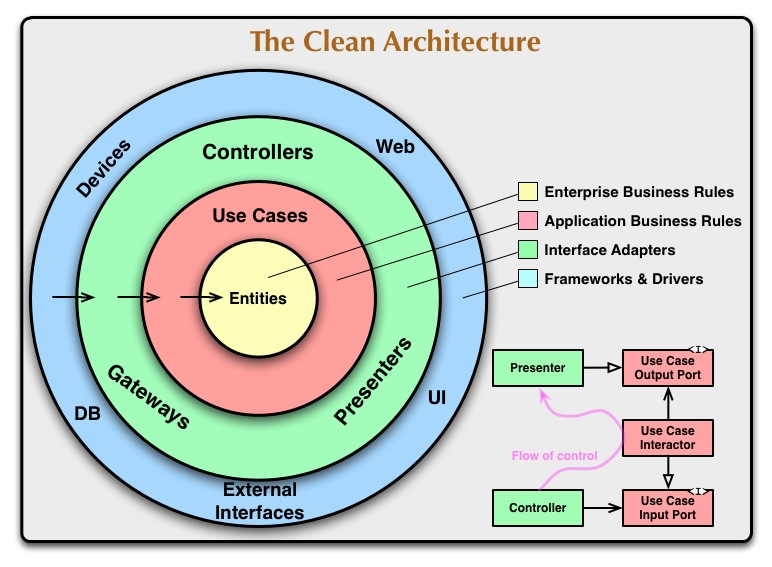
\includegraphics[width=0.9\textwidth]{graphics/CleanArchitecture.jpg}  
	\caption{Čistá architektura}
	\label{fig:clearch}
\end{figure}


Clean Architecture, česky \uv{Čistá architektura} je návrhový princip, který definuje strukturu softwarového systému tak, aby byla nezávislá na frameworku, UI, databázi a externích agentech. Díky oddělení byznysové logiky a technických detailů zajišťuje snadnou údržbu, testovatelnost a abstrakci mezi vrstvami.

Podle striktního pravidla závislostí (angl. The Dependency Rule) je směr vrstev definován do středu. Vnitřní vrstvy nemají povědomí o~tom, co se děje ve vnějších vrstvách.~\cite{clearch}

Architektura backendu se inspiruje principy Clean Architecture. Zdrojový kód je rozdělen do samostatných projektů pro doménové modely a rozhraní, aplikační logiku, infrastrukturu, datové přenosové objekty a prezentační vrstvu. Toto rozdělení omezuje přímé propojení případů užití s~konkrétní implementací databáze, Podmanu, RabbitMQ nebo GitHub~API a usnadňuje změnu jednotlivých technologií a další rozšiřování systému.

Architektura se skládá z~následujících vrstev:
\begin{itemize}
	\item \textbf{Doménová} (\textit{Domain}) se nachází v~samotném jádře architektury. Obsahuje základní doménové modely, výjimky a pravidla, která nejsou závislá na databázi, webovém rozhraní ani externích knihovnách.
	\item \textbf{Aplikační} (\textit{Application}) obsahuje případy užití systému a řídí průběh jednotlivých operací. V~systému InQuest zajišťuje například vytvoření požadavku na vyhodnocení, validaci vstupních údajů a zpracování přijatého výsledku.
	\item \textbf{Infrastrukturní} (\textit{Infrastructure}) implementuje komunikaci s~databází a externími službami. Patří sem například přístup k~databázi pomocí Entity Framework Core, řízení kontejnerů přes Podman, komunikace s~RabbitMQ a získávání údajů prostřednictvím GitHub~API.
	\item \textbf{Prezentační} (\textit{Presentation}): vystavuje koncové body pro komunikaci přes HTTP. Příjímá požadavky klienta, předává je aplikační vrstvě a převádí výsledky zpracování do odpovídajících HTTP odpovědí.
\end{itemize}

Konkrétní rozdělení backendové aplikace do uvedených vrstev a odpovědnosti jednotlivých projektů jsou popsány v~podkapitole~\ref{subsec:backend}.


\subsection{REST API}
\label{subsec:restapi}
Pro komunikaci klientských aplikací se systémem bylo zvoleno REST~API. Tento způsob komunikace umožňuje vystavit funkce backendu prostřednictvím HTTP rozhraní a oddělit tak implementaci serverové části od konkrétního uživatelského rozhraní. Systém může být díky tomu používán například prostřednictvím Swagger UI nebo být napojen na další interní aplikace společnosti.

REST (\textit{Representational State Transfer}) je architektonický styl určený pro návrh distribuovaných webových služeb. Komunikace probíhá pomocí protokolu HTTP a standardních metod, jako jsou \kiinlinecode{text}{!}{GET}, \kiinlinecode{text}{!}{POST}, \kiinlinecode{text}{!}{PUT} nebo \kiinlinecode{text}{!}{DELETE}.~\cite{restapi}

Jednou z~vlastností REST rozhraní je bezstavovost (\textit{stateless}). Každý požadavek musí obsahovat informace potřebné pro jeho samostatné zpracování a server nemusí mezi jednotlivými požadavky uchovávat stav klientské relace. To zjednodušuje komunikaci mezi klientem a backendem a umožňuje nezávislé zpracování požadavků.

V~systému InQuest slouží REST~API zejména k~vytvoření nového požadavku na vyhodnocení úlohy, získání jeho aktuálního stavu, načtení uložených výsledků a případnému opakování vyhodnocení. Samotná kontrola řešení probíhá asynchronně. API proto po přijetí požadavku nečeká na sestavení a spuštění odevzdaného projektu, ale vrátí klientovi informace o~vytvořeném záznamu. Výsledek lze následně získat samostatným požadavkem.


\subsection{Backend}
\label{subsec:backend}
Backendová aplikace je rozdělena do několika projektů, které odpovídají jednotlivým vrstvám Clean Architecture. Každá vrstva má vymezenou odpovědnost a s~ostatními částmi komunikuje prostřednictvím definovaných rozhraní. Díky tomu lze měnit implementaci infrastruktury nebo externích služeb bez zásahu do aplikační logiky.

\textbf{Prezentační vrstva} zajišťuje komunikaci mezi klientem a aplikační vrstvou prostřednictvím REST~API. Přijímá HTTP požadavky, provádí jejich základní kontrolu a předává je odpovídajícím aplikačním službám. Zároveň převádí výsledky zpracování do HTTP odpovědí.

V~této vrstvě se registrují služby využívané prostřednictvím dependency injection a inicializují se nástroje Swagger a Serilog. Swagger poskytuje interaktivní dokumentaci REST~API, zatímco Serilog slouží k~zaznamenávání informací o~průběhu zpracování požadavků a vzniklých chybách.

Projekt obsahuje složku \textit{Controllers}, ve které jsou definovány jednotlivé kontrolery a jejich endpointy. Složka \textit{Filters} obsahuje filtry určené pro zachytávání a jednotné zpracování výjimek. Převod mezi interními modely aplikace a datovými objekty vystavovanými prostřednictvím API zajišťují mapovací profily ve složce \textit{Mapper}.

\textbf{Projekt DTO} představuje unifikovaný datový kontrakt pro celý systém. DTO jsou reprezentovány jako třídy bez byznys logiky, které přenášejí data mezi jednotlivými vrstvami a externími systémy.

\textbf{Doménová vrstva} představuje vnitřní část aplikace a obsahuje základní modely systému, abstrakce služeb, vlastní výjimky a konfigurační objekty. Tato vrstva není závislá na webovém frameworku, databázi ani konkrétních externích službách. Ostatní vrstvy mohou využívat modely a rozhraní, která jsou v~ní definována. V~tomto specifickém systému jsou popsány modely pro abstrakce (rozhraní služeb), výjimky, nastavení a~tak.

\textbf{Aplikační vrstva} obsahuje orchestraci datových toků a validační logiku procesů. Jejím úkolem je například validace vstupních údajů, vytvoření požadavku na vyhodnocení a zpracování výsledku přijatého z~kontejnerového prostředí. Implementace je rozdělena do několika částí:

\begin{itemize}
	\item \textbf{\texttt{/AssignmentEvaluation}} obsahuje logiku spojenou se zahájením vyhodnocení úlohy. Zpracovává adresu GitHub repozitáře, ověřuje její platnost a prostřednictvím GitHub~API získává informace o~použitém programovacím jazyce.
	\item \textbf{\texttt{/Services}} je popis poskytovaných služeb.
	\begin{itemize}
		\item \texttt{Assignment}: spravuje životní cyklus požadavku a stav ukládá do databáze.
		\item \texttt{Result}: zpracovává výstup po vyhodnocení, rozdělí standardní výstup na informace o~sestavení a spuštění, nastavuje příznaky úspěchu a ukládá výsledek do databáze.
		\item \texttt{Value}: kontroluje hodnoty získané z~výstupu řešení uchazeče vůči očekávaným hodnotám. Pro každé zadání se modul mění.
	\end{itemize}
	\item \textbf{\texttt{/Validator}} je složka pro služby, které se týkají validace.
\end{itemize}

\textbf{Infrastrukturní vrstva} zajišťuje komunikaci s~databází a externími službami. Přístup k~databázi je realizován pomocí \textit{Entity Framework Core}. Komponenta \texttt{PodmanManager} komunikuje se službou Podman prostřednictvím jejího HTTP rozhraní a zajišťuje vytváření, spouštění, sledování a odstraňování kontejnerů.

Součástí infrastruktury je také napojení na \textit{RabbitMQ}, které zajišťuje asynchronní příjem výsledků z~jednotlivých kontejnerů a jejich předání aplikační vrstvě ke zpracování. Integrace s~\textit{GitHub~API} slouží k~ověření existence a dostupnosti repozitáře a k~získání informace o~jeho hlavním programovacím jazyce.

Takto navržené rozdělení odděluje hlavní logiku vyhodnocování od konkrétních technologií. Externí služby lze díky tomu upravit nebo nahradit, aniž by bylo nutné výrazně měnit případy užití definované v~aplikační vrstvě.


\subsection{Runners}
Runnery představují jednu z~nejdůležitějších částí systému InQuest. Zajišťují zpracování odevzdaných projektů, jejich sestavení a spuštění v~izolovaném kontejnerovém prostředí. Zároveň řeší jeden z~hlavních požadavků práce, kterým je podpora více programovacích jazyků bez nutnosti měnit hlavní logiku aplikace.

Při jejich návrhu bylo proto důležité oddělit společný průběh vyhodnocení od příkazů specifických pro jednotlivé programovací jazyky. Každý podporovaný jazyk využívá vlastní runner, jehož úkolem je ověřit strukturu odevzdaného projektu, provést jeho sestavení a následně jej spustit.

Jednotlivé runnery sdílejí společnou část implementace, která zajišťuje řízení celého procesu, práci se vstupními údaji a odeslání výsledku. Liší se pouze částí obsahující příkazy specifické pro konkrétní programovací jazyk. Díky tomuto rozdělení není nutné při přidání nového jazyka znovu implementovat celý průběh vyhodnocení.

Společná část runnerů obsahuje následující skripty:

\begin{itemize}
	\item \textbf{\texttt{checkVariables.sh}} je skript, který kontroluje přítomnost požadovaných vstupních údajů při startu kontejneru. Nejprve ověří, zda byla přiložena URL adresa ke GitHub repozitáři a poté jestli má kontejner přístup k~cestě pro access token v~Podman secrets. Token je nutný pro práci se soukromými repozitáři (a k~funkčnosti i s~veřejnými) a je do kontejneru předáván prostřednictvím mechanismu Podman Secrets.
	\item \textbf{\texttt{generateValidationResult.sh}} vytváří výstupní datovou strukturu obsahující informace o~průběhu a výsledku vyhodnocení. 

	\item \textbf{\texttt{reportResult.sh}} je skript, který výsledek odešle prostřednictvím RabbitMQ do zprávové fronty, odkud jej převezme backendová aplikace.
	\item \textbf{\texttt{validate.sh}} obsahuje hlavní logiku kontroly odevzdaného řešení. Zajišťuje stažení GitHub repozitáře, získání potřebných údajů o~projektu a spuštění jazykově specifického skriptu \texttt{start.sh}. Běh skriptu je omezen časovým limitem, aby nemohlo dojít k~nekonečnému zpracování například v~důsledku zablokovaného nebo chybně implementovaného programu.
	\item \textbf{\texttt{run.sh}} představuje hlavní vstupní bod runneru. Řídí pořadí jednotlivých kroků, spouští ostatní skripty a zajišťuje ukončení procesu po dokončení nebo vzniku chyby.
\end{itemize}

Konkrétní implementace pro jednotlivé programovací jazyky jsou umístěny ve složkách se zkratkou příslušného programovacího jazyka. Každá z~těchto složek využívá společné skripty a doplňuje je o~příkazy potřebné pro sestavení a spuštění projektu daného jazyka.

Každá jazyková složka obsahuje zejména následující soubory:

\begin{itemize}
	\item \textbf{\texttt{runnerScript-<language\_extension>.sh}} reprezentuje konkrétní implementaci daného jazyka. Ověřuje přítomnost povinných souborů v~projektu a spouští odpovídající příkazy technologie ke kompilaci a spuštění běhu.

	\item \textbf{\texttt{Dockerfile}} definuje předpis pro sestavení kontejnerového obrazu runneru. Přibalí se zde sdílené skripty a stáhnou se dodatečné systémové příkazy podle skriptu \texttt{../installPrerequisities.sh}. Jazykově specifický skript je při sestavení přejmenován na \texttt{start.sh} a jako vstupní bod kontejneru je nastaven skript \texttt{run.sh}.
\end{itemize}

Přidání podpory nového jazyka proto spočívá především ve vytvoření nové složky, definici odpovídajícího kontejnerového obrazu a implementaci jazykově specifického skriptu. Nový runner je dále nutné zaregistrovat v~souboru \linebreak{} \texttt{appsettings.json}, kde se uvede název jazyka, jméno obrazu a jeho verze. Pokud výstup nového jazyka nelze zpracovat univerzálním parserem, může být nutné upravit také třídu \texttt{ResultService}.

Tento návrh významně omezuje rozsah potřebných změn, přidání jazyka ale není úplně automatické a nemusí vždy spočívat pouze ve vytvoření nové složky v~\texttt{runners/}. Podrobný postup je uveden v~adresáři \texttt{./documentation} v~souboru \texttt{testRunnerDocumentation.md}.

\newpage

\section{Automatizované sestavení a nasazování}
Jelikož aplikace využívá větší množství kontejnerových obrazů a podporuje postupné rozšiřování o~nové programovací jazyky, bylo potřeba automatizovat proces sestavení a nasazení. Z~tohoto důvodu byla vytvořena CI/CD pipeline v~prostředí GitLab. Konfigurace je definována v~souboru \textbf{\texttt{.gitlab-ci.yml}}. Pipeline zajišťuje automatizované verzování, kompilaci backendu, přípravu Docker obrazů a dynamické sestavení izolovaných testovacích runnerů.

Pipeline je rozdělena do fází \textit{update}, \textit{build}, \textit{test}, \textit{deploy}, \textit{build-test-runners} a \textit{deploy-test-runners}. Jednotlivé úlohy pipeline používají v~názvu příponu \texttt{\_\_job}.

\begin{itemize}
	\item \textbf{update}: tato fáze přiděluje každému sestavení unikátní číslo verze odpovídající historii v~GitLabu. Skript nejdříve vyparsuje základní verzi ze souboru \texttt{Directory.Build.props}. K~této verzi se připojí identifikátor běžící pipeline. Výsledné číslo verze (např. 1.0.67) je pomocí \textbf{xmlstarlet} zpětně zapsáno do atributů \textit{AssemblyVersion} a \textit{PackageVersion} a následně předáno jako artefakt souboru \texttt{version.env} pro další úlohy. Díky tomu používají všechny sestavené části systému stejné číslo verze.

	\item \textbf{build} a \textbf{deploy}: zde se na základě definovaného \texttt{Dockerfile} sestaví obrazy aplikace s~tagem unikátního čísla verze získaného z~předchozího kroku a s~tagem \kiinlinecode{text}{!}{latest}. Tyto obrazy jsou poté ve fázi \textbf{deploy} nahrány do kontejnerového registru, odkud je lze následně stáhnout na cílový server a použít při nasazení aplikace.

	\item \textbf{build-test-runners} a \textbf{deploy-test-runners}: stejně jako fáze \textbf{build}, tato také sestavuje obrazy pro jednotlivé podporované programovací jazyky. Protože je systém navržen tak, aby bylo možné přidat nový jazyk vytvořením nové složky v~adresáři \texttt{runners}, byla obdobným způsobem navržena také CI/CD pipeline. Provádí následující operace:
	\begin{enumerate}
		\item Skript projde všechny podadresáře v~adresáři \texttt{./runners/}. Každý nalezený podadresář představuje implementaci runneru pro konkrétní programovací jazyk, například \texttt{cs}, \texttt{cpp} nebo \texttt{java}.
		\item Pro každý runner je načten příslušný soubor \texttt{Dockerfile}. Pomocí nástroje \kiinlinecode{text}{!}{sed} je z~instrukce \kiinlinecode{text}{!}{FROM ... AS final} získána verze použitého základního obrazu.
		\item Na základě názvu jazyka a získané verze je sestaven tag výsledného obrazu, například \texttt{test-runner-cs:8.0}.
		\item Pro každý nalezený jazyk je spuštěno sestavení kontejnerového obrazu.
		\item Dynamicky sestaví tag obrazu (např. test-runner-cs:8.0) a spustí \kiinlinecode{text}{!}{docker build}.
		\item Seznam nově vytvořených obrazů je uložen a předán další úloze, která zajistí jejich hromadné odeslání do registru. 
	\end{enumerate}
\end{itemize}

Současná CI/CD pipeline zajišťuje verzování, sestavení a publikování backendové aplikace a kontejnerových runnerů. V~konfiguraci je připravena také struktura pro fázi automatického testování, tato část zatím není implementována. V~budoucnu by bylo vhodné pipeline rozšířit o~spouštění jednotkových a integračních testů před sestavením a publikováním výsledných obrazů. Tím by bylo možné zachytit chyby před jejich nasazením a zabránit publikování nefunkční verze systému.

Pipeline tedy neobsahuje pevně zapsaný seznam podporovaných jazyků, ale zjišťuje jej přímo ze struktury adresáře \texttt{runners}. Tento přístup snižuje režii spojenou s~údržbou systému. Při nasazení podpory pro nový programovací jazyk není potřeba upravovat konfiguraci CI/CD pipeline, protože skript novou složku najde a zpracuje autonomně. 

\newpage


\section{Implementace}
Tato kapitola se věnuje průběhu hlavního procesu systému InQuest, který začíná přijetím požadavku na vyhodnocení a končí uložením výsledku do databáze. Zaměřuje se na spolupráci backendové aplikace, GitHub~API, kontejnerového prostředí Podman a zprávového brokeru RabbitMQ. 


\subsection{Průběh zpracování požadavku}

\begin{figure}[H]
	\centering
	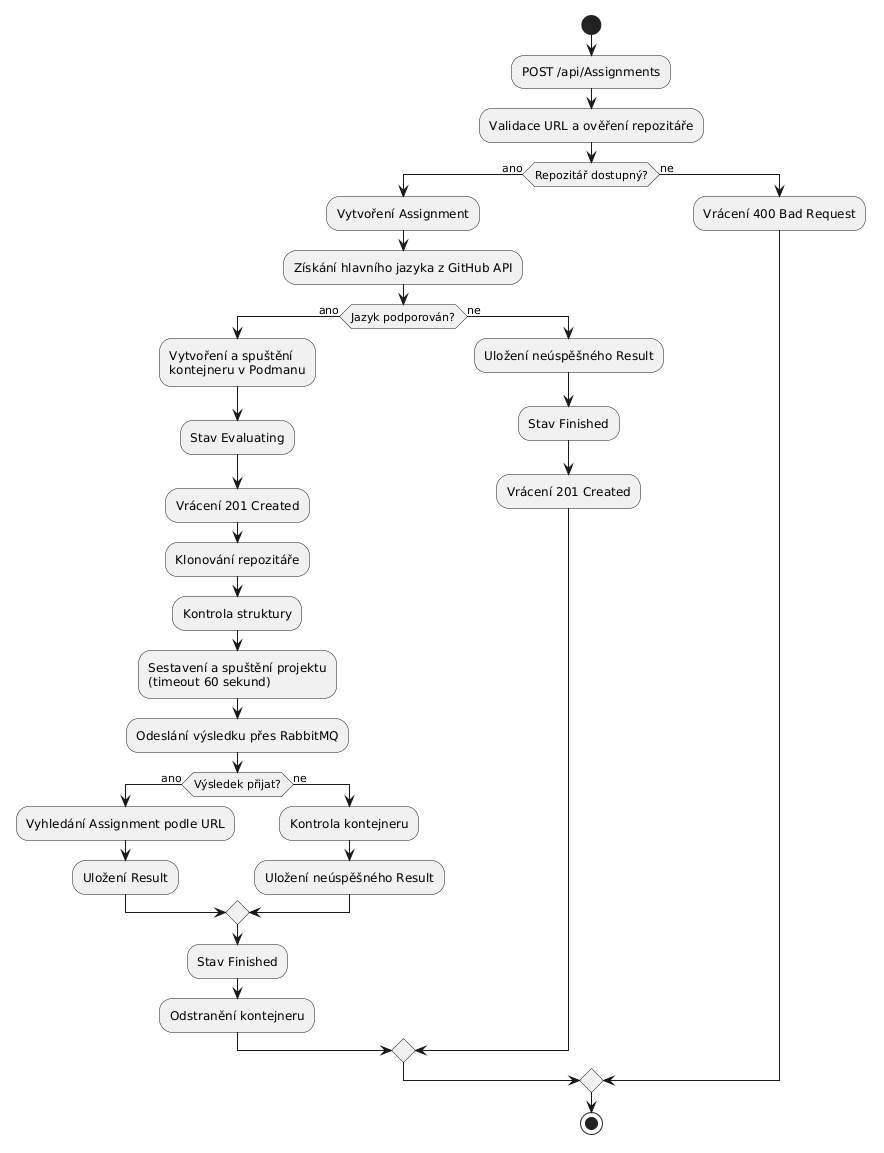
\includegraphics[width=0.9\textwidth]{graphics/ActivityDiagram.png}
	\caption{Průběh vyhodnocení programátorské úlohy}
	\label{fig:activityDiagram}
\end{figure}

Celkový průběh vyhodnocení programátorské úlohy je znázorněn na obrázku~\ref{fig:activityDiagram}. 

Proces začíná přijetím požadavku \kiinlinecode{text}{!}{POST /api/Assignments}, jehož tělo obsahuje URL adresu GitHub repozitáře. Backend ověří formát adresy a pomocí GitHub~API zkontroluje existenci a dostupnost repozitáře. Neplatná nebo nedostupná adresa vede k~odpovědi se stavovým kódem \kiinlinecode{text}{!}{400 Bad Request} a záznam není vytvořen.

Pro platnou adresu vytvoří backend v~databázi záznam typu \textit{Assignment}. Prostřednictvím GitHub~API získá seznam jazyků obsažených v~repozitáři a jako hlavní jazyk vybere jazyk s~největším množstvím zdrojového kódu. Pokud GitHub~API nevrátí žádný jazyk nebo pro zjištěný jazyk neexistuje runner, je k~zadání uložen neúspěšný výsledek a jeho stav je změněn na \kiinlinecode{text}{!}{Finished}. Požadavek i v~tomto případě vrací vytvořený záznam se stavovým kódem \kiinlinecode{text}{!}{201 Created}.

Pokud je jazyk podporován, backend vybere odpovídající kontejnerový obraz a prostřednictvím Podman~API vytvoří a spustí runner. Runner naklonuje repozitář, upraví názvy souborů podle pravidel validačního skriptu, ověří požadovanou strukturu projektu a spustí jazykově specifický skript.

Po spuštění kontejneru API nečeká na dokončení vyhodnocení. Klient obdrží vytvořený záznam a aktuální stav může následně získat samostatným požadavkem \kiinlinecode{text}{!}{GET}. Výsledek runner odešle asynchronně prostřednictvím RabbitMQ.


\subsection{Zpracování výsledku}
Po dokončení validace vytvoří runner výsledek obsahující informace o~průběhu kontroly, sestavení a spuštění projektu. Standardní a chybový výstup jazykově specifického skriptu jsou sloučeny do jediné textové hodnoty. Pomocné značky ve výstupu následně umožňují backendu rozlišit část týkající se sestavení a část vzniklou při spuštění programu.

Zpráva obsahuje URL repozitáře, identifikátor zpracovaného commitu, programovací jazyk, sloučený výstup a informace o~úspěšnosti validace. Po jejím přijetí backend vyhledá odpovídající záznam typu \textit{Assignment} podle URL repozitáře. Následně vytvoří záznam typu \textit{Result}, přiřadí jej k~nalezenému zadání a změní stav zadání na \kiinlinecode{text}{!}{Finished}.

Jazykově specifický skript má časový limit 60 sekund. Backend současně pravidelně kontroluje celkovou dobu existence kontejnerů. Pokud runner výsledek neodešle, kontejner překročí nastavený časový limit nebo skončí neočekávaným způsobem, backend uloží neúspěšný výsledek a kontejner odstraní.


\subsection{Datový model}
Datový model systému je tvořen dvěma hlavními entitami \texttt{AssignmentEntity} a \texttt{ResultEntity}. Jejich vztah je znázorněn na obrázku~\ref{fig:dataModel}.

\begin{figure}[h]
	\centering
	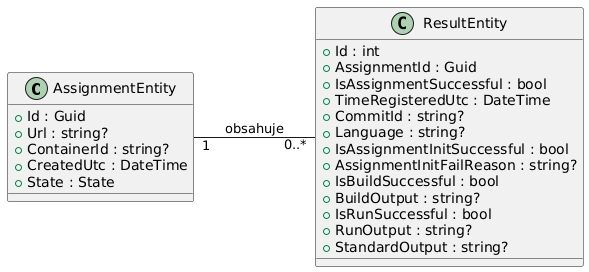
\includegraphics[width=0.9\textwidth]{graphics/EntityModels.png}
	\caption{Datový model systému InQuest}
	\label{fig:dataModel}
\end{figure}

Entita \texttt{AssignmentEntity} představuje jeden požadavek na vyhodnocení programátorské úlohy. Obsahuje identifikátor, adresu GitHub repozitáře, identifikátor spuštěného kontejneru, čas vytvoření požadavku a jeho aktuální stav. Identifikátor kontejneru je využíván zejména při sledování běžících vyhodnocení a při následném odstranění kontejneru.

Entita \texttt{ResultEntity} uchovává výsledek konkrétního vyhodnocení. Obsahuje informace o~úspěšnosti inicializace, sestavení a spuštění projektu, zaznamenané výstupy jednotlivých kroků, použitý programovací jazyk a identifikátor zpracovaného commitu. Atribut \kiinlinecode{text}{!}{AssignmentId} slouží jako cizí klíč odkazující na příslušný záznam \texttt{AssignmentEntity}.

Mezi entitami je vytvořena vazba jedna k~mnoha. Jeden záznam \linebreak{}\texttt{AssignmentEntity} může obsahovat nula až více záznamů \texttt{ResultEntity}. Díky tomu lze ke stejnému zadání ukládat výsledky opakovaných vyhodnocení a zachovat jejich historii.


\subsection{Implementace REST API}
REST~API zpřístupňuje hlavní případy užití systému klientským aplikacím. Nejdůležitější operace jsou uvedeny v~tabulce~\ref{tab:endpoints}.

\begin{table}[h]
	\centering
	\small
		\begin{tabular}{lll}
			\hline
			\textbf{Metoda} & \textbf{Endpoint} & \textbf{Význam} \\ \hline
			POST & \texttt{/api/Assignments} & Registrace požadavku na vyhodnocení \\ 
			GET & \texttt{/api/Assignments} & Získání všech uložených zadání  \\ 
			GET & \texttt{/api/Assignments/\{id\}} & Získání detailu konkrétního zadání \\
			PUT & \texttt{/api/Assignments} & Opakované vyhodnocení podle URL \\ 
			DELETE & \texttt{/api/Assignments/\{id\}} & Odstranění zadání z~databáze \\
			\hline
		\end{tabular}
	\caption{Vybrané endpointy systému}
	\label{tab:endpoints}
\end{table}

Požadavky \kiinlinecode{text}{!}{POST} a \kiinlinecode{text}{!}{PUT} přijímají objekt obsahující URL repozitáře. Opakované vyhodnocení se tedy nevyhledává podle identifikátoru v~adrese endpointu, ale podle URL předané v~těle požadavku.

\newpage


\section{Budoucí rozšíření}
Navržený systém byl vytvořen s~důrazem na modularitu a snadnou rozšiřitelnost. Současná implementace splňuje stanovené požadavky, nicméně architektura umožňuje další rozvoj, který může zvýšit kvalitu systému, usnadnit jeho údržbu a rozšířit možnosti jeho využití.

\begin{itemize}
	\item \textbf{Náhrada služby GitHub Classroom}:
	V~průběhu dokončování práce bylo oznámeno ukončení služby GitHub Classroom k~28.~srpnu 2026~\cite{githubclasssupp}. GitHub Classroom byl ve společnosti využíván pro vytváření soukromých repozitářů, do kterých uchazeči odevzdávali vypracované úlohy.

	Ukončení této služby nemá přímý vliv na hlavní funkce systému InQuest, protože systém pracuje s~běžnými GitHub repozitáři prostřednictvím jejich URL a GitHub~API. V~budoucnu ale bude nutné nahradit způsob, kterým jsou repozitáře pro jednotlivé uchazeče automaticky vytvářeny, nastavovány jako soukromé a předávány účastníkům náborového procesu. Samotný proces vyhodnocení může zůstat beze změny, pokud nové řešení zachová odevzdávání úloh prostřednictvím GitHub repozitářů.

	\item \textbf{Možnost nastavení očekávaného výsledku}:
	Současná implementace používá validační pravidla definovaná přímo v~systému. V~budoucnu by bylo vhodné umožnit zadavateli úlohy nastavit očekávaný výsledek, podle kterého má být odevzdané řešení vyhodnoceno. Tím by bylo možné systém využít pro větší množství různých zadání bez nutnosti upravovat validační logiku v~aplikačním kódu. 

	\item \textbf{Automatizované testování v~CI/CD}:
	Současná CI/CD pipeline zajišťuje sestavení aplikace a vytvoření kontejnerových obrazů. V~budoucnu by bylo vhodné pipeline rozšířit o~fázi, která zajišťuje automatické spouštění testů před samotným sestavením a nasazením aplikace. Díky tomu by bylo možné zachytit případné chyby během vývojového procesu a zabránit nasazení nefunkčních verzí systému.
	
	\item \textbf{Podpora dalších programovacích jazyků}:
	Architektura systému byla navržena tak, aby bylo možné jednoduše přidávat podporu dalších programovacích jazyků. Rozšíření spočívá především ve vytvoření nového runneru obsahujícího odpovídající kontejnerový obraz a skript definující proces sestavení a spuštění projektu. V~současné verzi systém podporuje jazyky \csharp{}, \cpp{}, Java, Python, Rust a JavaScript.
	
	\item \textbf{Rozšíření REST API a správa dat}:
	Stávající REST rozhraní se zaměřuje na základní životní cyklus jednotlivých požadavků. Pro usnadnění správy a integraci s~rozsáhlejšími systémy by bylo v~budoucnosti vhodné API rozšířit o~nové endpointy:
	
	\begin{itemize}
		\item \textbf{Hromadné zpracování požadavků (\kiinlinecode{text}{!}{POST /api/batch}):} Umožnilo by odeslat pole odkazů na repozitáře v~jediném HTTP požadavku rozhraní. Systém by následně hromadně vytvořil frontu úloh pro spuštění v~runneru, což by zjednodušilo obsluhu pro větší počet úloh naráz.
		\item \textbf{Správa a promazávání dat (\kiinlinecode{text}{!}{DELETE /api/all}):} Administrátorský endpoint určený k~hromadnému mazání historických záznamů a výsledků (případně s~možností filtrů podle data či stavu). To by usnadnilo údržbu databáze a uvolňování místa na disku.
	\end{itemize}
\end{itemize}

\newpage


%% Závěry práce. V jazyce práce a anglicky. Text pro jiný než
%% nastavený jazyk práce (nepovinným parametrem language makra
%% \documentclass, výchozí český) se zadává použitím makra s uvedením
%% jazyka jako nepovinného parametru.
\begin{kiconclusions}
Cílem bakalářské práce bylo navrhnout a implementovat systém InQuest pro automatizované vyhodnocování programátorských úloh. Navržené řešení přijímá odkaz na GitHub repozitář, zjistí použitý programovací jazyk, spustí odevzdaný projekt v~izolovaném kontejnerovém prostředí a uloží výsledek vyhodnocení.

Backendová aplikace byla navržena podle principů Clean Architecture a implementována na platformě .NET. Nedůvěryhodný zdrojový kód je spuštěn v~izolovaném kontejnerovém prostředí spravovaném pomocí Podmanu, zatímco výsledky jsou asynchronně předávány pomocí RabbitMQ. Důležitou součástí řešení jsou samostatné runnery pro jednotlivé programovací jazyky, které umožňují systém dále rozšiřovat bez výrazných změn hlavní aplikační logiky.

Výsledkem práce je funkční prototyp, který omezuje ruční práci mentorů, sjednocuje způsob zpracování odevzdaných úloh a snižuje rizika spojená se spouštěním nedůvěryhodného kódu. Stanovený cíl práce byl naplněn, přesto existuje prostor pro zlepšení.
\end{kiconclusions}

\begin{kiconclusions}[english]
The aim of this bachelor's thesis was to design and implement the InQuest system for automated evaluation of programming assignments. The proposed solution accepts a link to a GitHub repository, detects the programming language used, runs the submitted project in an isolated container environment and saves the evaluation result.

The backend application was designed according to the principles of Clean Architecture and implemented on the .NET platform. The untrusted source code is executed in an isolated container environment managed by Podman, while the results are transmitted asynchronously using RabbitMQ. An important part of the solution is the use of separate runners for individual programming languages, which allow the system to be further expanded without significant changes to the main application logic.

The result of the thesis is a functional prototype that reduces the amount of manual work required from mentors, unifies the processing of submitted assignments and reduces the risks associated with running untrusted code. The defined objective of the thesis was achieved, though there is still room for improvement.
\end{kiconclusions}


%% Přílohy obsahu textu práce, za makrem \appendix.
\appendix

%% Obsah elektronických dat. Poslední příloha. Upravte podle vlastní
%% práce!
\section{Obsah elektronických dat} 
\label{sec:ObsahData}

Přiložená elektronická data obsahují:

\begin{description}

\item[\texttt{text/}] \hfill \\
  Adresář s~textem práce ve formátu PDF, vytvořený s~použitím
  závazného stylu KI PřF UP v~Olomouci pro závěrečné práce, včetně
  všech (textových) příloh, a všechny soubory potřebné pro
  bezproblémové vytvoření PDF dokumentu textu (případně v~ZIP
  archivu), tj.~zdrojový text textu a příloh, vložené obrázky, apod.


\item[\texttt{README.md}] \hfill \\
  Dokumentace požadavků a postupu sestavení, nasazení, konfigurace a 
  spuštění systému InQuest.


\item[\texttt{inquest/}] \hfill \\
  Adresář se zdrojovými soubory implementovaného systému InQuest. 


\item[\texttt{test\_zadani/}] \hfill \\
  Adresář obsahující zjednodušenou podobu programátorského zadání 
  použitého při testování systému InQuest.

\end{description}


%% -------------------------------------------------------------------

%% Sazba volitelného seznamu zkratek, za přílohami.
%\printglossary

%% Sazba povinné bibliografie, za přílohami (případně i za seznamem
%% zkratek). Při použití BibLaTeXu použijte makro
%% \printbibliography. jinak prostředí thebibliography. Ne obojí!

%% Sazba i v textu necitovaných zdrojů, při použití
%% BibLaTeXu. Volitelné.
%\nocite{*}

%% Vlastní sazba bibliografie při použití BibLaTeXu.

%% Bibliografie, včetně sazby, při NEpoužití BibLaTeXu.
 %\begin{thebibliography}{9}

 %\end{thebibliography}

\printbibliography

%% Sazba volitelného rejstříku, za bibliografií.


\printindex

\end{document}

%%% Local Variables:
%%% mode: latex
%%% TeX-master: t
%%% End:
